

\begin{frame}[ctb!]
  \frametitle{Heat Limits In Geology}
  % table?
  Important heat limits in materials of the repository restrict loading designs 
  and capacity.
   \begin{table}[h!]
    \centering
    \footnotesize{
    \begin{tabular}{|l|c|c|l|}
      \multicolumn{4}{c}{\textbf{Models of Heat Load for Various Geologies}}\\
      \hline
      Source & Nation & Geology & Methodology \\  
      (Who) & (Where) & (What) & (How) \\  
      \hline
      Enresa \cite{von_lensa_red-impact_2008}           & Spain       & Granite       &  CODE\_BRIGHT 3D Finite Element \\ 
      NRI   \cite{von_lensa_red-impact_2008}            & Czech Rep.  & Granite       &  Specific Temperature Integral   \\
      ANDRA \cite{andra_granite:_2005}                  & France      & Granite       &  3D Finite Element CGM code   \\
      SKB \cite{ab_long-term_2006}                      & Sweden      & metagranite   &  1D-3D Site  Descriptive Models \\
      SCK$\cdot$CEN   \cite{von_lensa_red-impact_2008}  & Belgium     & Clay          &  Specific Temperature Integral   \\ 
      ANDRA \cite{andra_argile:_2005}                   & France      & Argile Clay   &  3D Finite Element CGM code   \\
      NAGRA \cite{johnson_project_2002, johnson_calculations_2002}  & Switzerland  & Opalinus Clay &  3D Finite Element CGM code \\
      GRS \cite{von_lensa_red-impact_2008}              & Germany     & Salt          &  HEATING (3D finite difference)   \\ 
      NCSU(Li)   \cite{li_examining_2007}               & USA         & Yucca Tuff    &  Specific Temperature Integral \\        
      NCSU(Nicholson) \cite{nicholson_thermal_2007}     & USA         & Yucca Tuff    &  COSMOL 3D Finite Element\\
      Radel \& Wilson \cite{radel_repository_2007}      & USA         & Yucca Tuff    &  Specific Temperature Change \\ 
      \hline
    \end{tabular}
    \caption[Models for Heat Transport for Various Geologies]{Methods by which to calculate heat 
    load are independent of geology. Maximum heat load constraints, however, vary among host formations. }
    \label{tab:heat}
    }
  \end{table}

\end{frame}

% heat based capacity 
\begin{frame}[ctb!]
  \frametitle{Impact of Repository Designs}
  % lines, points, infinite lines, footprints.
   \begin{table}[h!]
  \centering
      \footnotesize{
      \begin{tabular}{|l|c|c|r|}
          \multicolumn{4}{c}{\textbf{Yucca Mountain Footprint Expansion Calculations}}\\
          \hline
          Author&Max. Capacity&Footprint&Details\\
          &$tonnes$&$km^2$&\\
          \hline
          &&&\\
          OCRWM&$70,000$&$4.65$&``statutory case''\\
          &$97,000$&$6$&``full inventory case''\\
          &$119,000$&$~7$&``additional case''\\
          \hline
          &&&\\
          Yim, M.S.&$75,187$&$4.6$&SRTA code\\
          &$76,493$&$4.6$&STI method\\
          &$95,970$&$4.6$&$63$m drift spacing\\
          &$82,110$&$4.6$&75 yrs. cooling\\
          \hline
          &&&\\
          Nicholson, M.&$103,600$&$4.6$&drift spacing\\
          \hline
          &&&\\
          EPRI&&&\\
          &$63,000$&$6.5$&Base Case CSNF\\
          option 1&$126,000$&$13$&expanded footprint\\
          option 2&$189,000$&$6.5$&multi-level design\\
          option 3&$189,000$&$6.5$&grouped drifts\\
          options 2+3&$252,000$&$6.5$&hybrid\\
          options 1+(2or3) &$378,000$&$13$&hybrid\\
          options 1+2+3 &$567,000$&$13$&hybrid\\
          \hline
        \end{tabular}
        \caption[Yucca Mountain Footprint Expansion Calculations]{Various analyses based on heat 
        load limited repository designs have resulted in footprint expansion calculations of the 
        YMR.} 
        \label{tab:footprint}
        }
      \end{table}

   \begin{figure}[h!]
     \begin{center}
       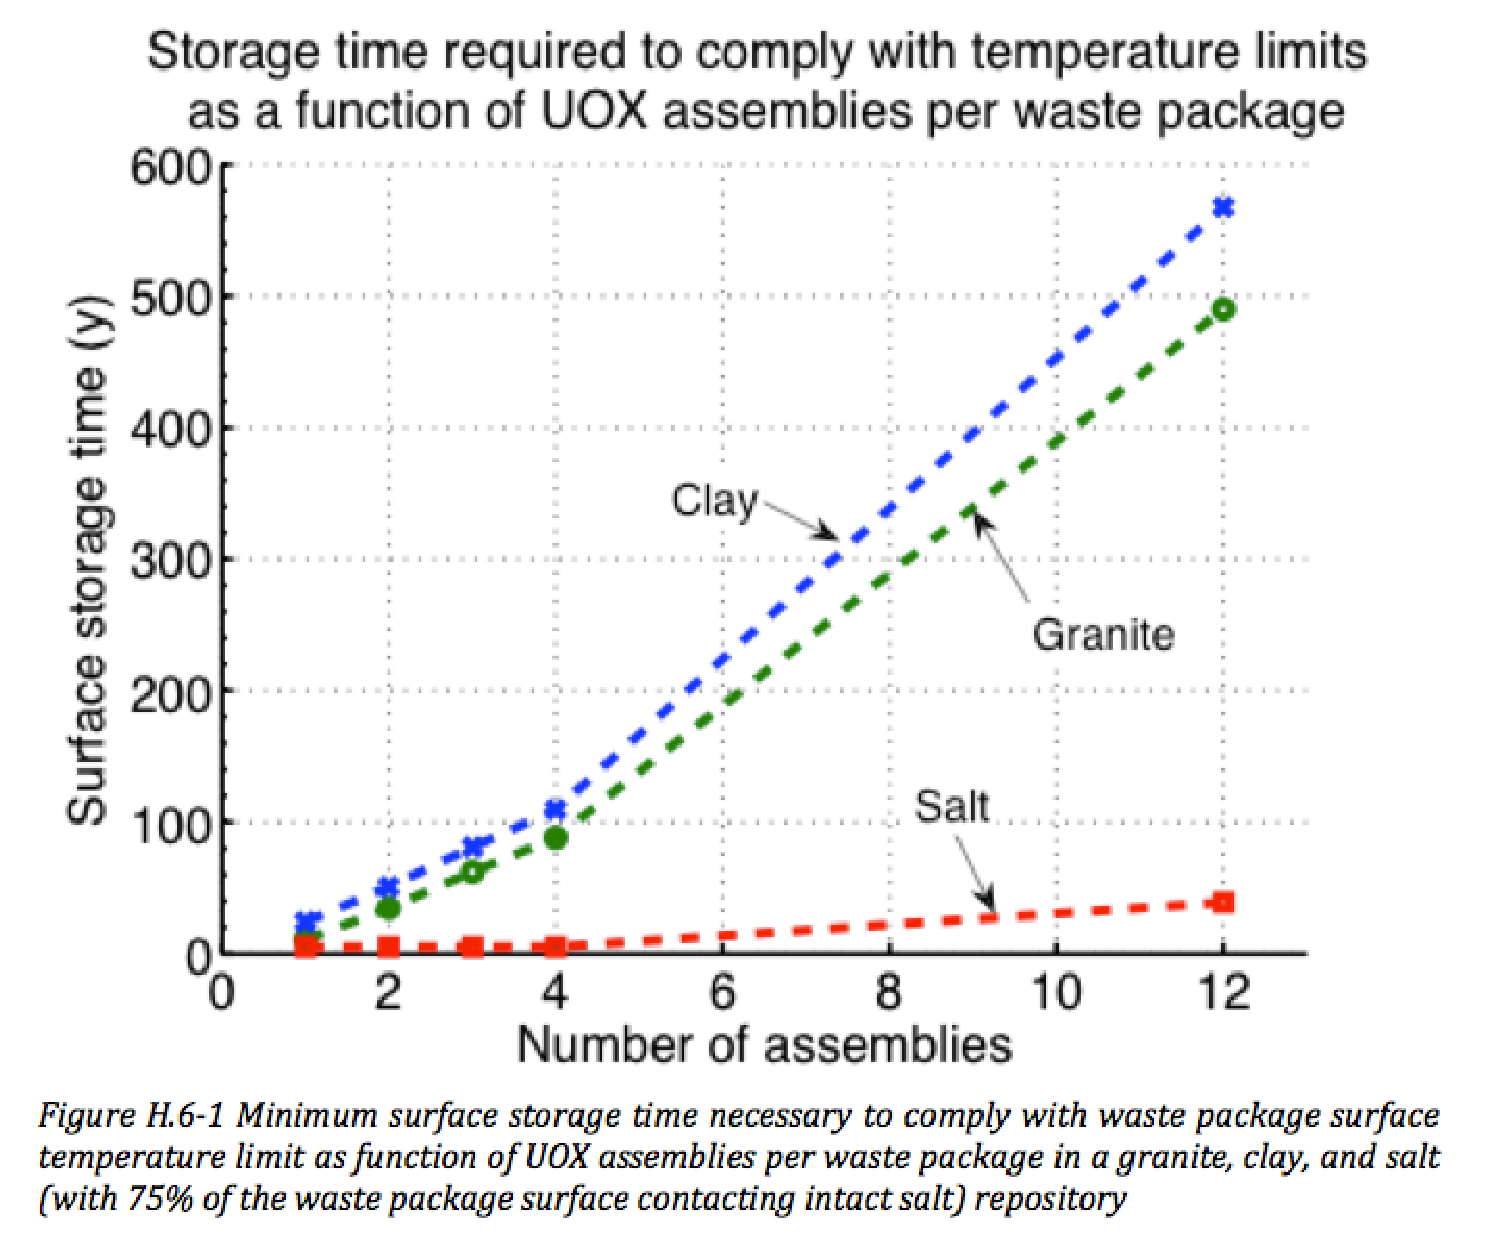
\includegraphics[height=.5\textheight]{llnlGeos.eps}
     \end{center}
     \caption{LLNL has found that the higher heat limit, alcove geometry, and 
     high conductivity in salt allows for earlier loading times.}
     \label{fig:llnlGeos}
   \end{figure}
\end{frame}

\begin{frame}[ctb!]
  \frametitle{Detailed Techniques}
  % 2d,3d,finite diffs, etc.
   \begin{table}[h!]
    \centering
    \footnotesize{
    \begin{tabular}{|l|c|c|l|}
      \multicolumn{4}{c}{\textbf{Models of Heat Load for Various Geologies}}\\
      \hline
      Source & Nation & Geology & Methodology \\  
      (Who) & (Where) & (What) & (How) \\  
      \hline
      Enresa \cite{von_lensa_red-impact_2008}           & Spain       & Granite       &  CODE\_BRIGHT 3D Finite Element \\ 
      NRI   \cite{von_lensa_red-impact_2008}            & Czech Rep.  & Granite       &  Specific Temperature Integral   \\
      ANDRA \cite{andra_granite:_2005}                  & France      & Granite       &  3D Finite Element CGM code   \\
      SKB \cite{ab_long-term_2006}                      & Sweden      & metagranite   &  1D-3D Site  Descriptive Models \\
      SCK$\cdot$CEN   \cite{von_lensa_red-impact_2008}  & Belgium     & Clay          &  Specific Temperature Integral   \\ 
      ANDRA \cite{andra_argile:_2005}                   & France      & Argile Clay   &  3D Finite Element CGM code   \\
      NAGRA \cite{johnson_project_2002, johnson_calculations_2002}  & Switzerland  & Opalinus Clay &  3D Finite Element CGM code \\
      GRS \cite{von_lensa_red-impact_2008}              & Germany     & Salt          &  HEATING (3D finite difference)   \\ 
      NCSU(Li)   \cite{li_examining_2007}               & USA         & Yucca Tuff    &  Specific Temperature Integral \\        
      NCSU(Nicholson) \cite{nicholson_thermal_2007}     & USA         & Yucca Tuff    &  COSMOL 3D Finite Element\\
      Radel \& Wilson \cite{radel_repository_2007}      & USA         & Yucca Tuff    &  Specific Temperature Change \\ 
      \hline
    \end{tabular}
    \caption[Models for Heat Transport for Various Geologies]{Methods by which to calculate heat 
    load are independent of geology. Maximum heat load constraints, however, vary among host formations. }
    \label{tab:heat}
    }
  \end{table}

  Similar heat transport models can be used for all geologies, but are 
  differentiated by material parameters $(c_p, K, \rho)$ and different 
  thermal constraints.
\end{frame}
